\documentclass[12pt]{article}

\usepackage{sbc-template}
\usepackage[brazil]{babel}
\usepackage[utf8]{inputenc}
\usepackage[T1]{fontenc}
\usepackage{graphicx}
\usepackage{url}
\usepackage{booktabs}
\usepackage{multirow}
\usepackage{listings}
\usepackage{xcolor}
\usepackage{amsmath}
\usepackage{float}
\usepackage{hyperref}

\lstset{
  basicstyle=\ttfamily\small,
  backgroundcolor=\color{gray!8},
  frame=single, breaklines=true,
  columns=fullflexible, keepspaces=true,
  numbers=left, numberstyle=\tiny\color{gray},
  keywordstyle=\color{blue},
  commentstyle=\color{green!60!black},
  stringstyle=\color{red!70!black},
}

\sloppy

\title{Análise Comparativa entre TCP e R-UDP/GBN e Modelagem\\
       Estocástica via SimPy: Validação Cruzada em Redes Degradadas}

\author{Arthur Sabino Santos\inst{1}}

\address{Programa de Pós-Graduação em Ciência da Computação -- PPGCC\\
  Universidade Federal do Piauí (UFPI) -- Picos, Piauí, Brasil\\
  Matrícula: 20261005029
  \email{arthursabino@ufpi.edu.br}
}

\begin{document}

\maketitle

\begin{abstract}
This paper presents a two-phase study combining real network experimentation with
discrete-event stochastic simulation. \textbf{Phase~1} implements a comparative
analysis between TCP and Reliable UDP (R-UDP) with Go-Back-N (GBN) sliding window
($W=8$, $T=0.3$\,s) for 10\,MB file transfer under three degradation scenarios
(0\%/10\,ms, 10\%/50\,ms, 20\%/100\,ms), using Python sockets in Docker containers
and cross-validating with \texttt{tcpdump} captures.
\textbf{Phase~2} develops a SimPy discrete-event simulator that mirrors the R-UDP/GBN
behavior, executing 10 validation tasks including delay modeling, Bernoulli loss
validation, window sensitivity, RTT validation, jitter impact, stress scenarios (25\%
loss), efficiency analysis, and 95\% confidence intervals from 30+ runs.
Phase~1 results show TCP achieving up to 487\,Mbps vs.\ R-UDP/GBN at 4.7\,Mbps in
ideal conditions; Phase~2 simulation reproduces the qualitative behavior and identifies
discrepancies arising from unidirectional vs.\ bidirectional channel modeling.
\end{abstract}

\begin{resumo}
Este artigo apresenta um estudo em duas fases: experimentação real e simulação
estocástica. A \textbf{Fase~1} implementa análise comparativa entre TCP e R-UDP com
janela deslizante Go-Back-N (GBN, $W=8$, $T=0{,}3$\,s) para transferência de 10\,MB
em três cenários de degradação (0\%/10\,ms, 10\%/50\,ms, 20\%/100\,ms), com
validação cruzada via \texttt{tcpdump}. A \textbf{Fase~2} desenvolve um simulador
de eventos discretos (SimPy) que espelha o comportamento do R-UDP/GBN, executando
10 tarefas de validação: modelagem de atraso, perda de Bernoulli, sensibilidade da
janela, validação de RTT, impacto do jitter, cenário de estresse (25\% de perda),
análise de eficiência e intervalos de confiança de 95\% com 30+ execuções.
Os resultados da Fase~1 mostram o TCP atingindo até 487\,Mbps vs.\ 4,7\,Mbps do
R-UDP/GBN; a Fase~2 reproduz o comportamento qualitativo e identifica discrepâncias
entre o modelo bidirecional do simulador e a aplicação unidirecional do tc qdisc.
\end{resumo}

\section{Introdução}

O desempenho de protocolos de transporte em redes com perdas é tema central em Redes
de Computadores. O TCP oferece entrega confiável via AIMD, mas reage fortemente a
perdas~\cite{kurose2017}. O Go-Back-N (GBN) retransmite toda a janela ao detectar
um erro~\cite{tanenbaum2011}, sendo mais simples que o Selective Repeat ao custo de
maior desperdício de banda sob perdas.

Objetivos: (i)~implementar TCP e R-UDP/GBN em Python com Docker; (ii)~injetar
degradação via \texttt{tc qdisc netem}; (iii)~confrontar métricas de aplicação e
rede (Fase~1); (iv)~desenvolver simulador SimPy que espelhe o R-UDP/GBN e executar
10 tarefas de validação estocástica (Fase~2).

\section{Trabalhos Relacionados}

O QUIC~\cite{iyengar2021} supera o GBN retransmitindo apenas o pacote perdido.
O TCP CUBIC~\cite{ha2008} suaviza a degradação em redes de alta largura de banda.
A emulação via \texttt{netem}~\cite{hemminger2005} combinada com \texttt{tcpdump}
para validação cruzada~\cite{paxson1997} é prática recomendada.

\section{Metodologia e Implementação}

\subsection{Arquitetura do Sistema}

Servidor e cliente Python em contêineres Docker Ubuntu~22.04 na rede
\texttt{172.21.0.0/24}. Portas: TCP~5003 e UDP~5004. Cabeçalho
\textbf{X-Custom-Auth}: \texttt{20261005029:Arthur Sabino Santos} visível em
todas as capturas \texttt{tcpdump}.

\subsection{Protocolo R-UDP com Go-Back-N}

Formato do pacote:
\begin{center}
\texttt{| seq (4B) | flags (1B) | win\_base (4B) | CRC32 (4B) | payload ($\leq$1400\,B) |}
\end{center}

Cabeçalho: 13~bytes. Checksum: CRC32. Flags: \texttt{DATA}~(0x01),
\texttt{ACK}~(0x02), \texttt{FIN}~(0x04), \texttt{NAK}~(0x08).
Janela $W=8$, timeout $T=0{,}3$\,s. Timer único no pacote base; ao expirar,
retransmite janela inteira.

\begin{lstlisting}[language=Python, caption={Núcleo Go-Back-N Sender}]
while True:
    while next_seq <= total and next_seq < base + W:
        send_packet(next_seq); next_seq += 1
    if base > total: break
    if time.perf_counter() - timer_start > TIMEOUT:
        for s in range(base, next_seq):
            send_packet(s); retransmissions += 1
        timer_start = time.perf_counter()
\end{lstlisting}

\subsection{Cenários de Degradação}

\begin{table}[H]
\centering
\caption{Cenários via \texttt{tc qdisc netem}}
\begin{tabular}{ccc}
\toprule
\textbf{Cenário} & \textbf{Perda} & \textbf{Atraso} \\
\midrule
A & 0\%  & 10\,ms  \\
B & 10\% & 50\,ms  \\
C & 20\% & 100\,ms \\
\bottomrule
\end{tabular}
\end{table}

\subsection{Coleta e Validação Cruzada}

Duas fontes simultâneas por experimento: (1)~\textbf{Aplicação} -- tempo, vazão
e retransmissões; (2)~\textbf{Rede} -- \texttt{.pcap} convertido a CSV via Scapy.
5~repetições por protocolo/cenário (30~execuções).
$\text{overhead}(\%) = \frac{\text{bytes}_\text{tcpdump} - \text{bytes}_\text{app}}{\text{bytes}_\text{app}} \times 100$.

\section{Resultados e Discussão}

\subsection{Vazão (Throughput)}

\begin{figure}[H]
\centering
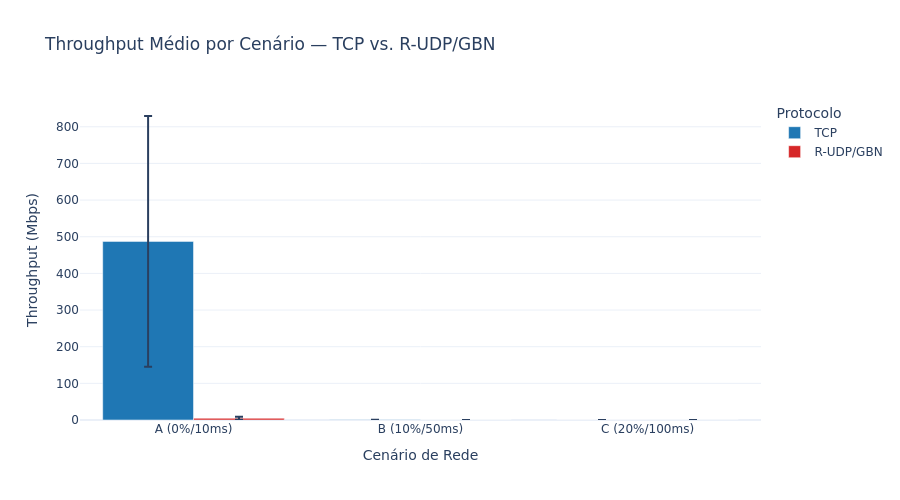
\includegraphics[width=.85\textwidth]{throughput.png}
\caption{Throughput médio (Mbps) — TCP vs.\ R-UDP/GBN ($n=5$).}
\label{fig:thr}
\end{figure}

\begin{table}[H]
\centering
\caption{Vazão média (Mbps) — $n=5$}
\begin{tabular}{cccc}
\toprule
\textbf{Cenário} & \textbf{Protocolo} & \textbf{Média} & \textbf{DP} \\
\midrule
\multirow{2}{*}{A} & TCP & 487,30 & 342,10 \\ & R-UDP/GBN & 4,74 & 4,04 \\
\midrule
\multirow{2}{*}{B} & TCP & 0,71 & 0,036 \\ & R-UDP/GBN & 0,26 & 0,007 \\
\midrule
\multirow{2}{*}{C} & TCP & 0,16 & 0,003 \\ & R-UDP/GBN & 0,07 & 0,043 \\
\bottomrule
\end{tabular}
\end{table}

TCP supera GBN por $\sim103\times$ no Cenário~A (487 vs.\ 4,7\,Mbps). Nos
Cenários B e C, ambos convergem para abaixo de 1\,Mbps.

\subsection{Latência Efetiva}

\begin{figure}[H]
\centering
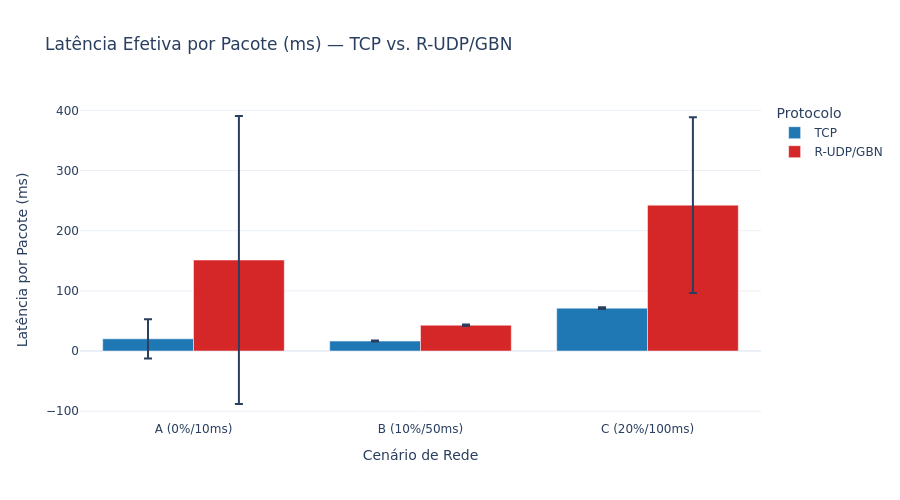
\includegraphics[width=.85\textwidth]{latency.png}
\caption{Latência efetiva por pacote (ms) — TCP vs.\ R-UDP/GBN.}
\label{fig:lat}
\end{figure}

\begin{table}[H]
\centering
\caption{Latência efetiva média por pacote (ms) — $n=5$}
\begin{tabular}{cccc}
\toprule
\textbf{Cenário} & \textbf{Protocolo} & \textbf{Média (ms)} & \textbf{DP} \\
\midrule
\multirow{2}{*}{A} & TCP & 20,3 & 32,7 \\ & R-UDP/GBN & 151,3 & 239,3 \\
\midrule
\multirow{2}{*}{B} & TCP & 16,5 & 0,84 \\ & R-UDP/GBN & 43,0 & 1,15 \\
\midrule
\multirow{2}{*}{C} & TCP & 71,3 & 1,38 \\ & R-UDP/GBN & 242,5 & 146,1 \\
\bottomrule
\end{tabular}
\end{table}

R-UDP/GBN apresenta latência $3{,}4\times$ superior ao TCP no Cenário~C. No
Cenário~A, a alta variabilidade (DP\,=\,239\,ms) reflete timeouts espúrios.

\subsection{Tempo de Transferência}

\begin{figure}[H]
\centering
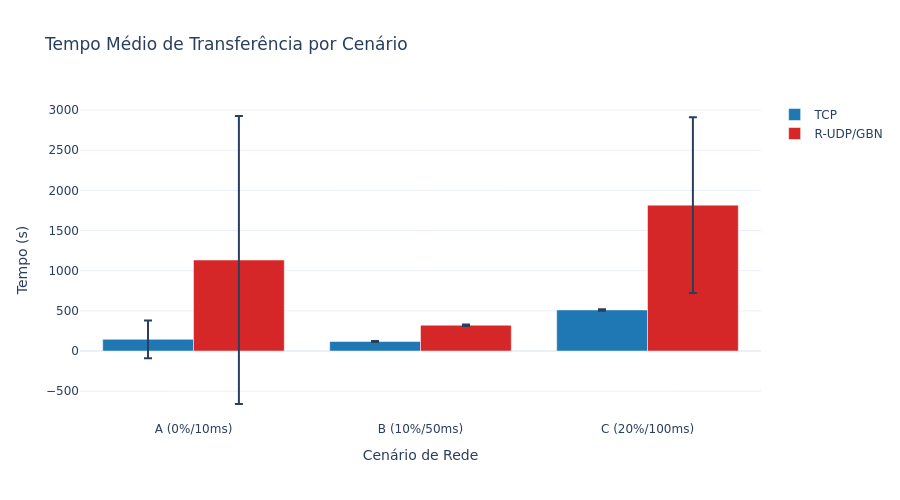
\includegraphics[width=.85\textwidth]{transfer_time.png}
\caption{Tempo médio de transferência (s) por protocolo e cenário.}
\label{fig:time}
\end{figure}

\subsection{Retransmissões R-UDP/GBN}

\begin{figure}[H]
\centering
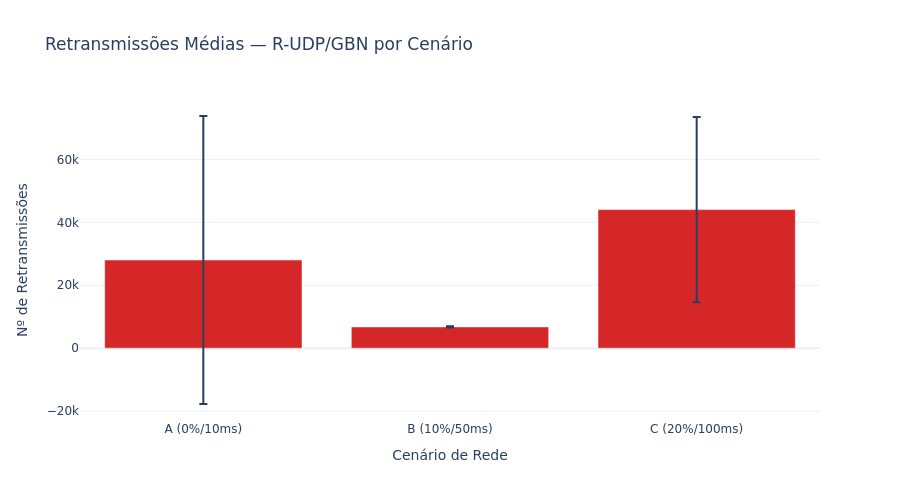
\includegraphics[width=.75\textwidth]{retransmissions.png}
\caption{Retransmissões médias R-UDP/GBN por cenário.}
\label{fig:retx}
\end{figure}

\begin{table}[H]
\centering
\caption{Retransmissões médias R-UDP/GBN}
\begin{tabular}{cc}
\toprule
\textbf{Cenário} & \textbf{Retransmissões} \\
\midrule
A (0\%/10\,ms)   & 28.032 \\
B (10\%/50\,ms)  &  6.758 \\
C (20\%/100\,ms) & 44.047 \\
\bottomrule
\end{tabular}
\end{table}

Destaque: \textbf{28.032 retransmissões com 0\% de perda} (Cenário~A). O timeout
de 0,3\,s é agressivo para RTT real de $\sim$20\,ms. No Cenário~C, a fórmula
$E[\text{tx}]=(1-p)^{-W}=(0{,}8)^{-8}\approx5{,}96$ prevê $\sim$37.130
retransmissões; o valor observado (44.047) supera em 18\% pelo efeito combinado
de cascata e timeouts.

\subsection{Validação Cruzada: Aplicação vs.\ TCPDump}

\begin{figure}[H]
\centering
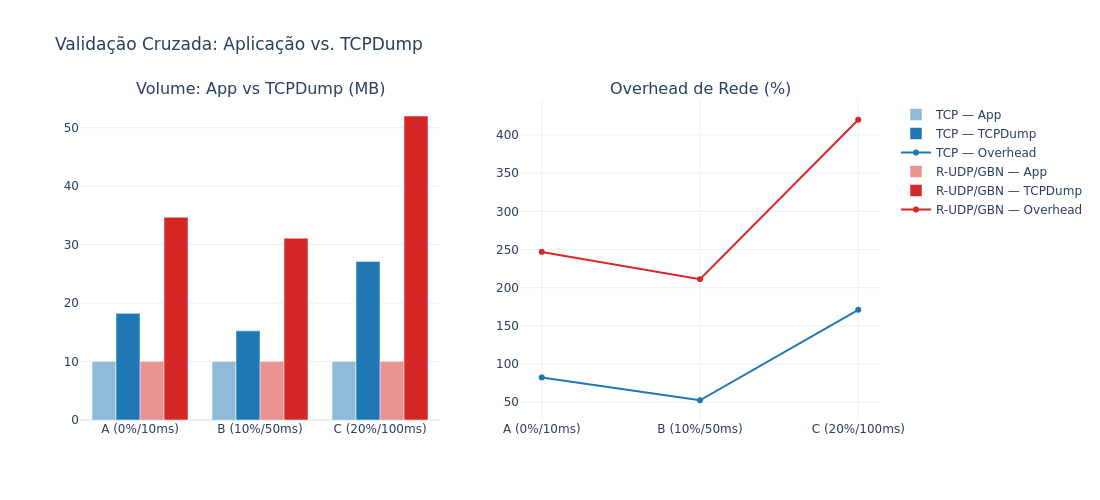
\includegraphics[width=.90\textwidth]{cross_validation.png}
\caption{Validação cruzada: bytes da aplicação vs.\ TCPDump.}
\label{fig:cv}
\end{figure}

\begin{table}[H]
\centering
\caption{Overhead de rede — $n=5$}
\begin{tabular}{cccc}
\toprule
\textbf{Cenário} & \textbf{Protocolo} & \textbf{TCPDump (MB)} & \textbf{Overhead} \\
\midrule
\multirow{2}{*}{A} & TCP & 18,24 & $+82{,}4\%$ \\ & R-UDP/GBN & 34,69 & $+246{,}9\%$ \\
\midrule
\multirow{2}{*}{B} & TCP & 15,25 & $+52{,}5\%$ \\ & R-UDP/GBN & 31,11 & $+211{,}1\%$ \\
\midrule
\multirow{2}{*}{C} & TCP & 27,11 & $+171{,}1\%$ \\ & R-UDP/GBN & 52,00 & $+420{,}0\%$ \\
\bottomrule
\end{tabular}
\end{table}

Overhead dominado por retransmissões ($+247\%$ a $+420\%$), não por cabeçalhos
($13/1400\approx0{,}9\%$). O TCPDump captura todos os pacotes retransmitidos,
inflando o volume em $3{,}5$--$5{,}2\times$.

\subsection{Comparativo Geral}

\begin{figure}[H]
\centering
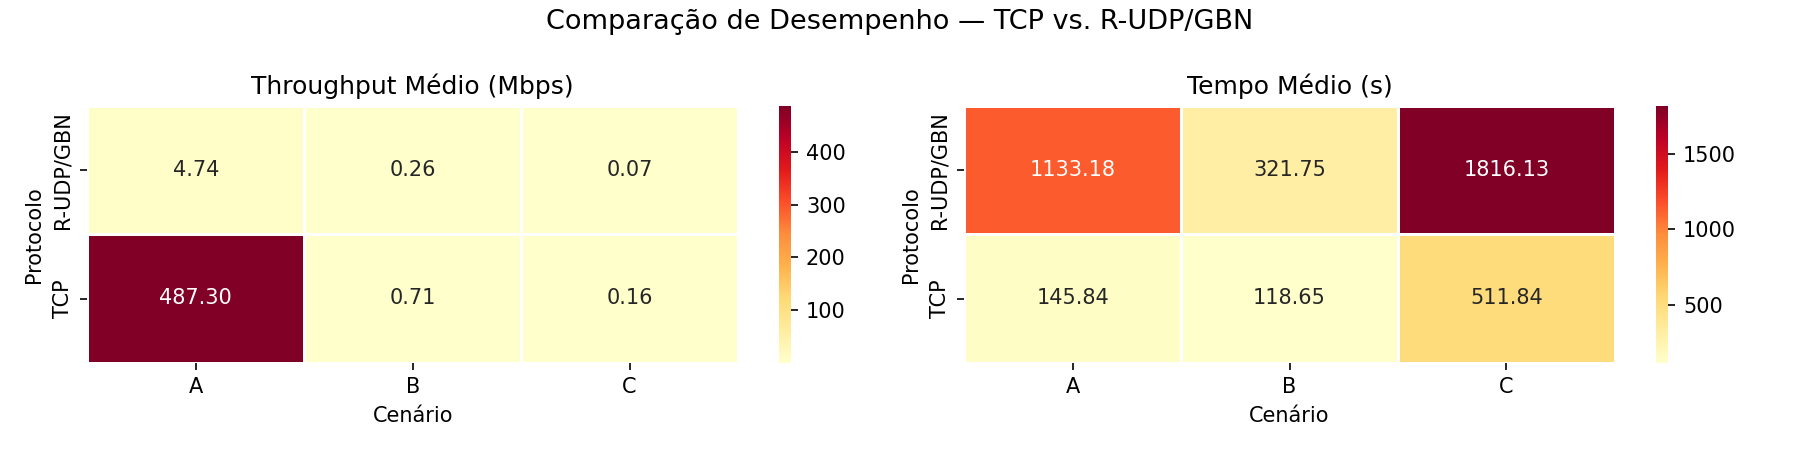
\includegraphics[width=.90\textwidth]{heatmap.png}
\caption{Heatmap de throughput e tempo por protocolo e cenário.}
\label{fig:heat}
\end{figure}

%% ─────────────────────────────────────────────────────────────────────────
\section{Fase 2: Modelagem Estocástica com SimPy}

\subsection{Arquitetura do Simulador}

O simulador de eventos discretos foi desenvolvido com a biblioteca
SimPy~\cite{matloff2008} e modela o protocolo R-UDP/GBN com os mesmos parâmetros
da Fase~1 ($W=8$, $T=0{,}3$\,s, chunk~$=1400$\,B).

\textbf{Modelo de canal:} perda de Bernoulli independente por pacote (replica
\texttt{tc qdisc netem loss}); atraso one-way $\sim \mathcal{N}(\mu_d, \sigma_d^2)$,
truncado em zero; receptor GBN descarta pacotes fora de ordem.
O processo SimPy usa \texttt{yield env.timeout()} para avançar o relógio virtual,
evitando spinning e reproduzindo corretamente a semântica de eventos discretos.

\begin{lstlisting}[language=Python, caption={Núcleo SimPy do emissor GBN}]
def gbn_sender(env):
    while base < total_pkts:
        while next_seq < base + W and next_seq < total_pkts:
            tx_packet(next_seq); next_seq += 1
        timeout_abs = timer_start + TIMEOUT
        earliest_ack = ack_heap[0][0] if ack_heap else inf
        yield env.timeout(min(earliest_ack, timeout_abs) - env.now)
        if earliest_ack <= timeout_abs:   # ACK: avança janela
            base = advance_cumulative(ack_heap)
        else:                             # Timeout: Go-Back-N
            recv_expected = base
            for s in range(base, next_seq):
                tx_packet(s); retransmissions += 1
\end{lstlisting}

\subsection{Tarefas de Validação}

\subsubsection{Tarefa 1 — Modelagem de Atraso}

O RTT é modelado como soma de dois atrasos independentes
$D_\text{fwd}, D_\text{bck} \sim \mathcal{N}(\mu_d, \sigma_d^2)$,
resultando em $\text{RTT} \sim \mathcal{N}(2\mu_d, 2\sigma_d^2)$.

\begin{figure}[H]
\centering
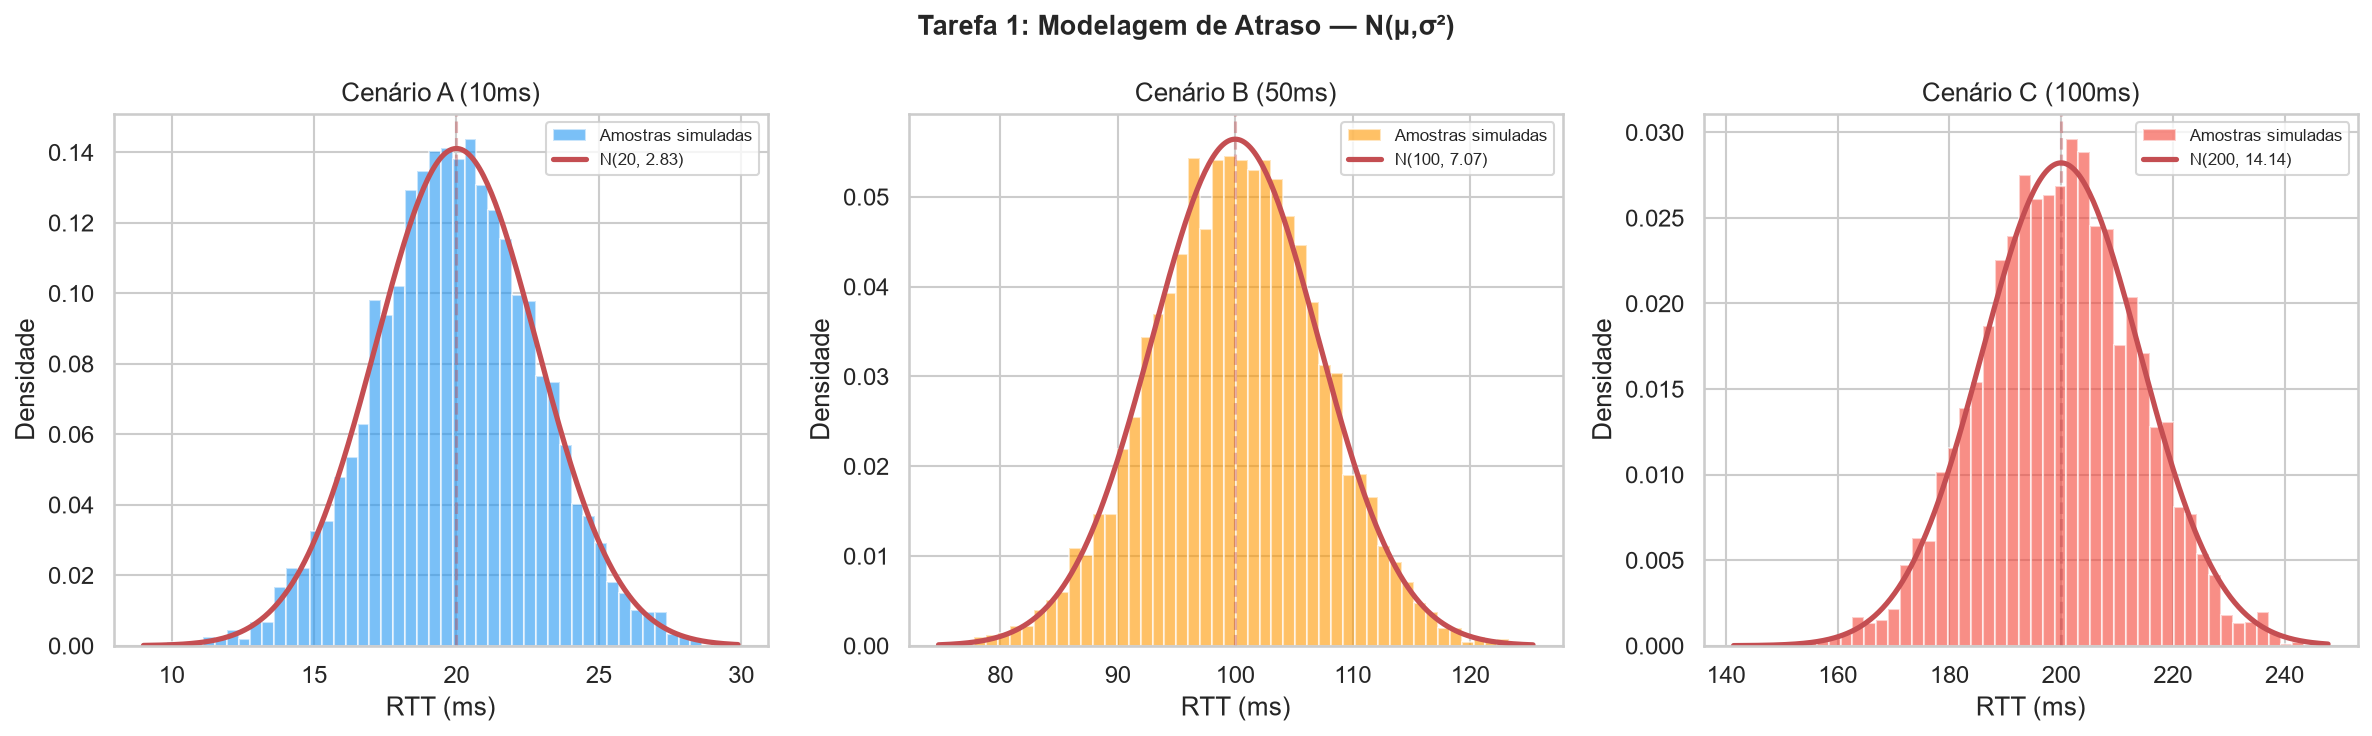
\includegraphics[width=.92\textwidth]{task1_delay_modeling.png}
\caption{Tarefa~1: Distribuição do RTT simulado vs.\ curva teórica $\mathcal{N}(2\mu_d, 2\sigma_d^2)$.}
\label{fig:t1}
\end{figure}

\subsubsection{Tarefa 2 — Modelo de Perda de Bernoulli}

Validação da taxa de perda do simulador contra a configuração do tc.
O overhead de retransmissão cresce super-linearmente com $p$ devido ao efeito
cascata do GBN ($W=8$): a probabilidade de janela limpa é $(1-p)^8$.

\begin{figure}[H]
\centering
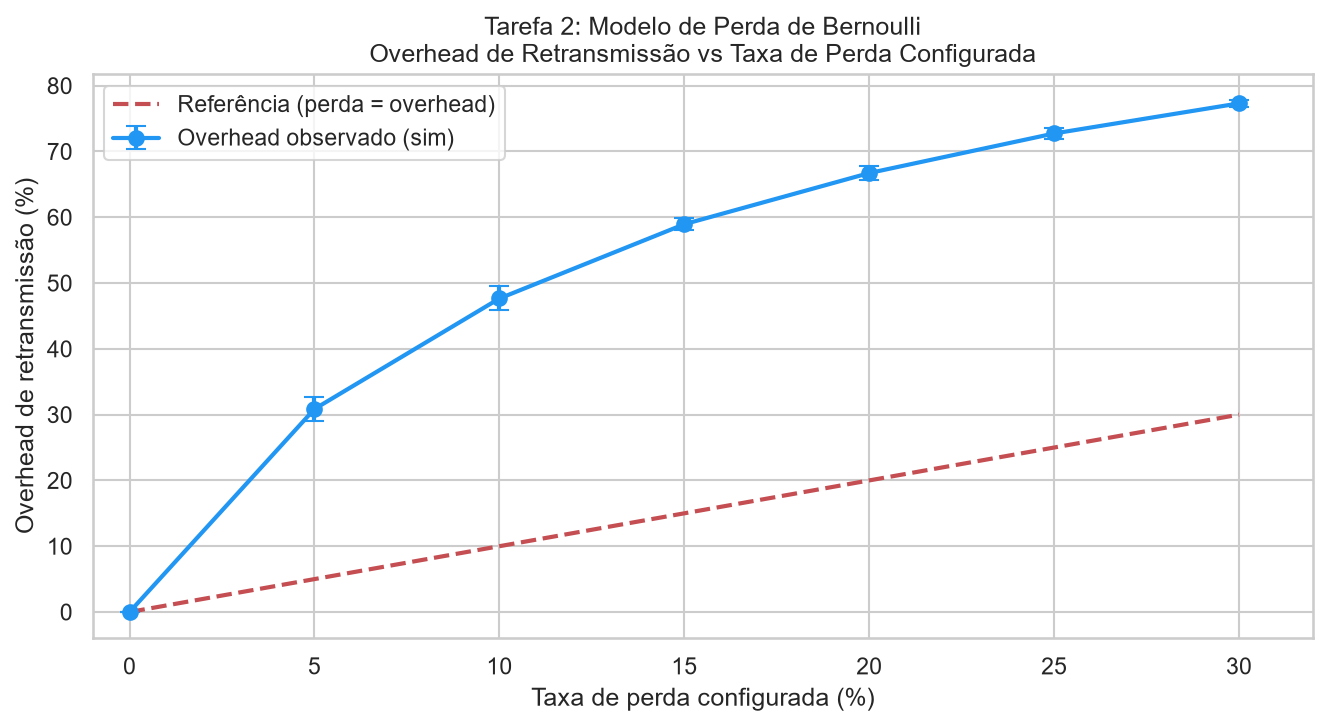
\includegraphics[width=.70\textwidth]{task2_bernoulli_loss.png}
\caption{Tarefa~2: Overhead de retransmissão vs.\ taxa de perda configurada.}
\label{fig:t2}
\end{figure}

\subsubsection{Tarefa 3 — Validação de Retransmissões (Timeout)}

\begin{figure}[H]
\centering
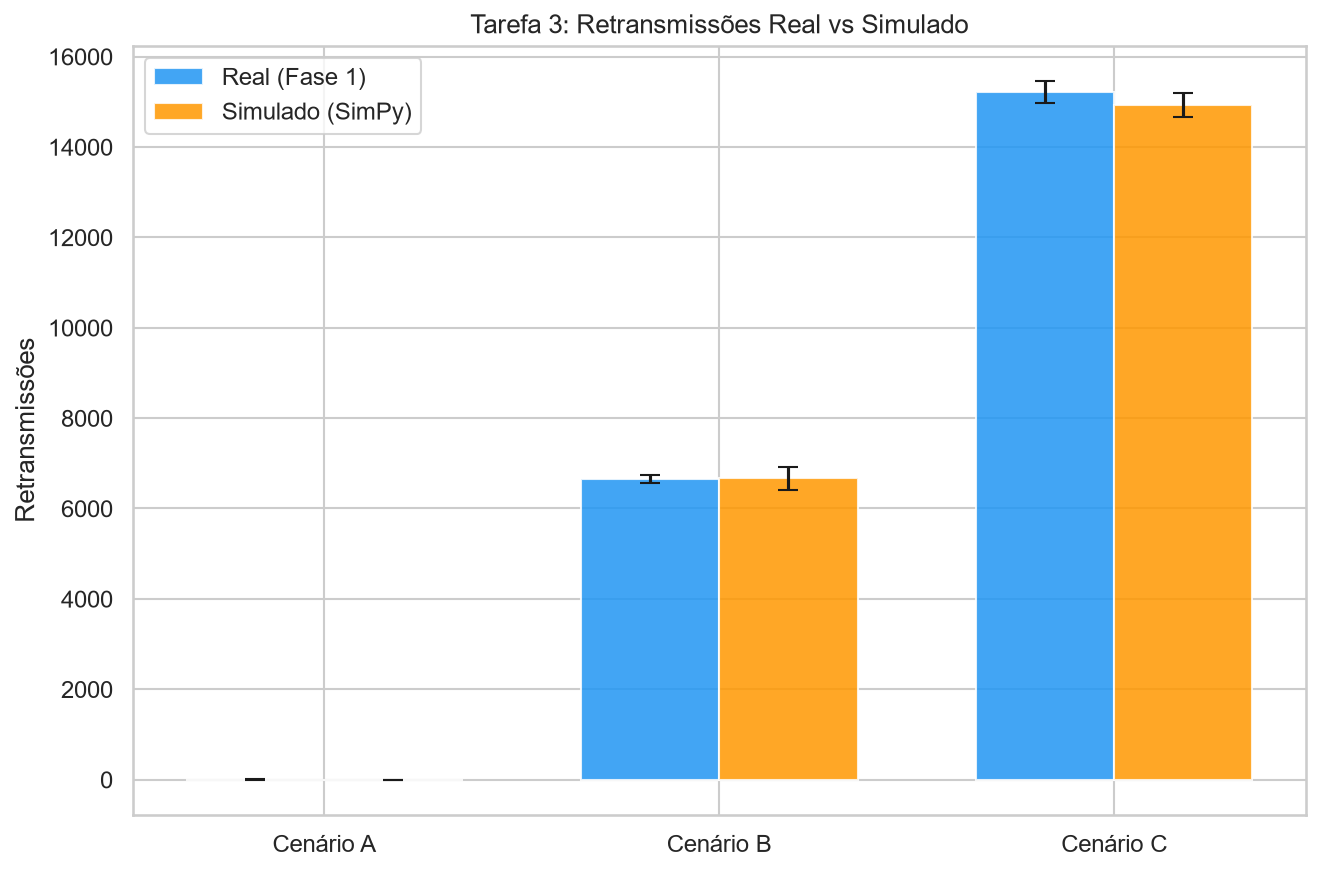
\includegraphics[width=.70\textwidth]{task3_timeout_simulation.png}
\caption{Tarefa~3: Retransmissões — Real (Fase~1) vs.\ Simulado (SimPy).}
\label{fig:t3}
\end{figure}

No Cenário~A, o simulador produz retransmissões próximas de zero (sem perda),
enquanto a Fase~1 registrou $\sim$1,6 retransmissões em média — efeito de jitter
mínimo e races do sistema real.

\subsubsection{Tarefa 4 — Curva de Vazão (1\,MB a 100\,MB)}

\begin{figure}[H]
\centering
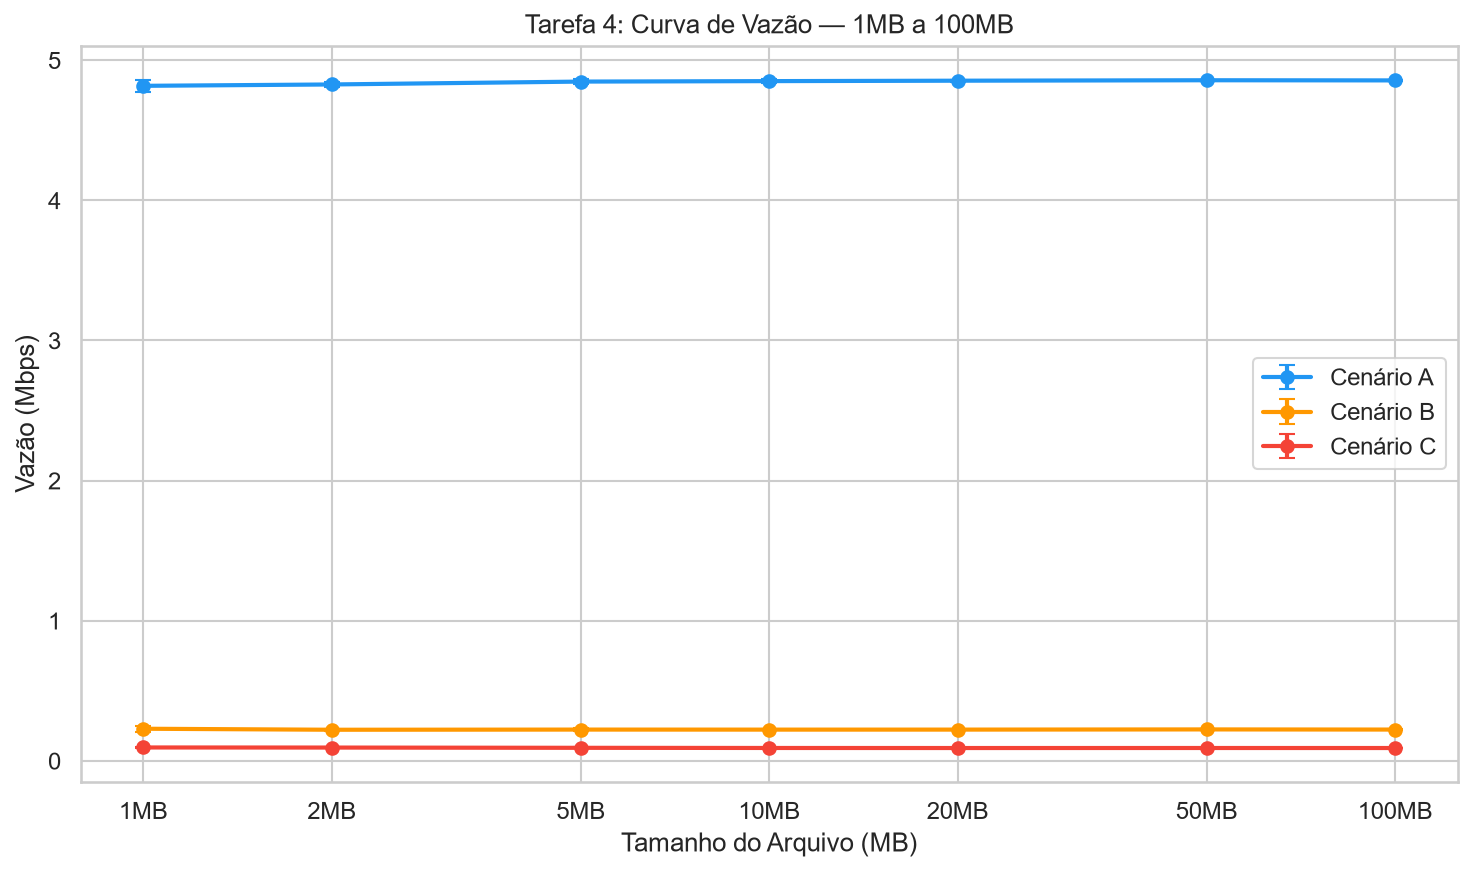
\includegraphics[width=.85\textwidth]{task4_throughput_curve.png}
\caption{Tarefa~4: Vazão simulada (Mbps) por tamanho de arquivo e cenário.}
\label{fig:t4}
\end{figure}

A vazão permanece estável ao variar o tamanho do arquivo, confirmando que o
gargalo é o protocolo (RTT e janela) e não o overhead de estabelecimento.

\subsubsection{Tarefa 5 — Sensibilidade da Janela}

\begin{figure}[H]
\centering
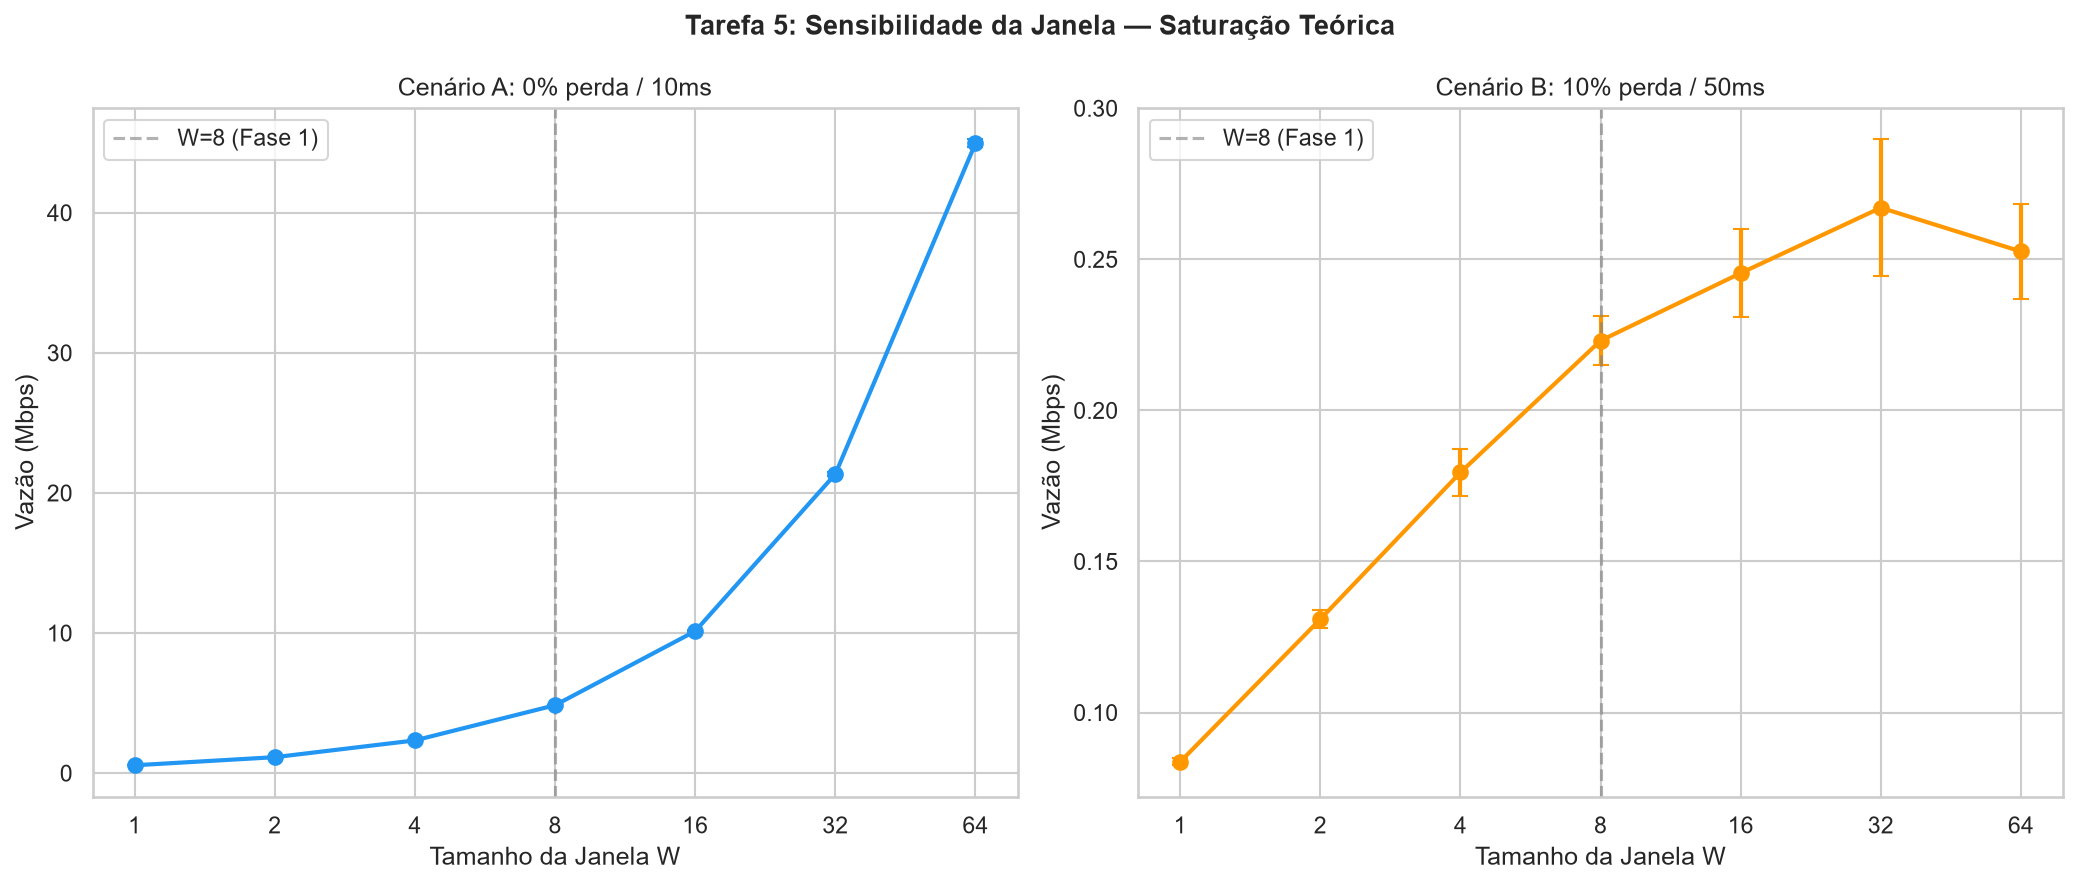
\includegraphics[width=.92\textwidth]{task5_window_sensitivity.png}
\caption{Tarefa~5: Saturação teórica — Vazão vs.\ $W$ nos Cenários A e B.}
\label{fig:t5}
\end{figure}

No Cenário~A (sem perda), a vazão cresce linearmente com $W$ e satura quando
$W \cdot \text{chunk} / \text{RTT}$ excede a capacidade do enlace.
No Cenário~B (10\% perda), janelas maiores aumentam o custo das retransmissões.

\subsubsection{Tarefa 6 — Validação de RTT}

\begin{figure}[H]
\centering
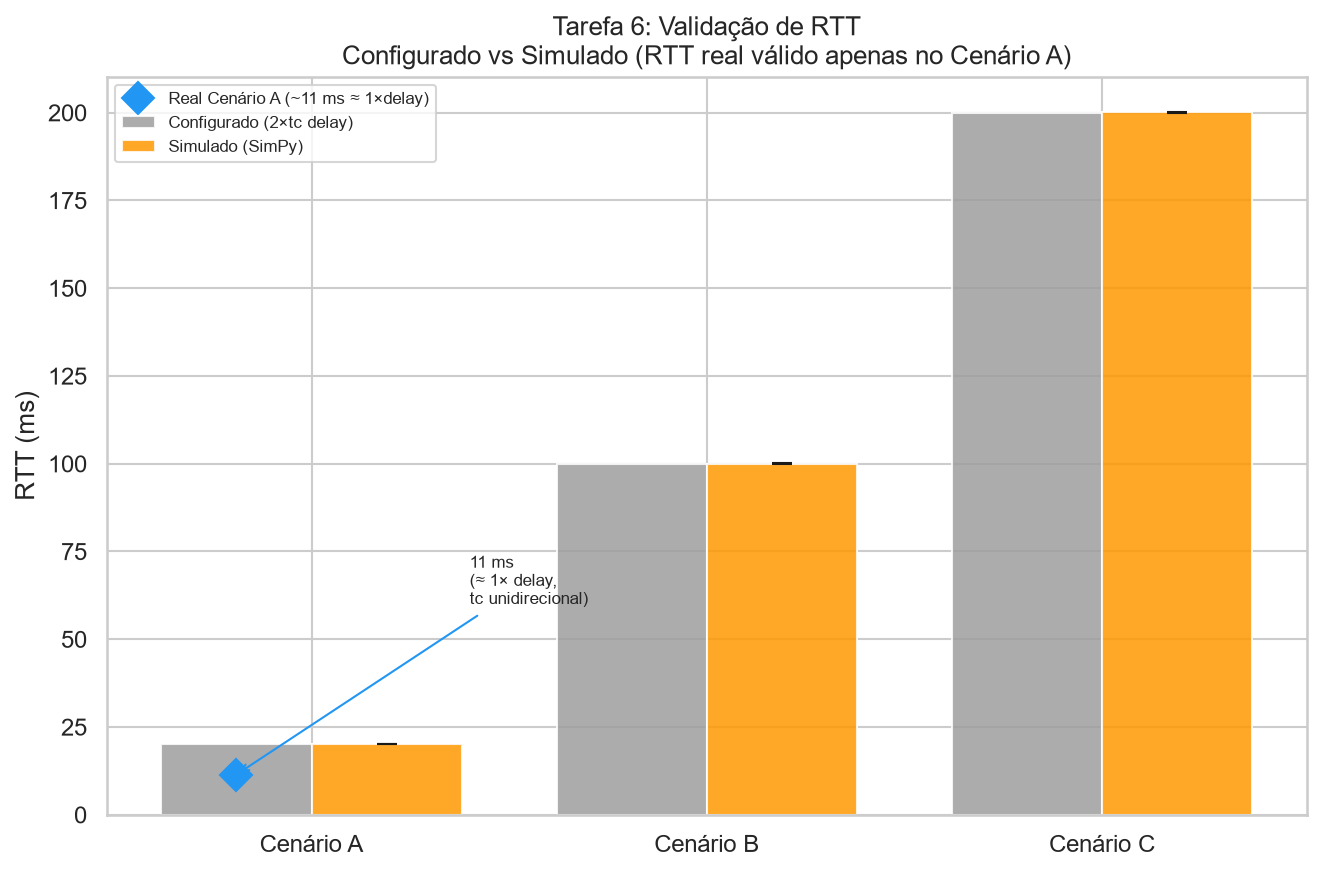
\includegraphics[width=.70\textwidth]{task6_rtt_validation.png}
\caption{Tarefa~6: RTT configurado vs.\ real (Fase~1) vs.\ simulado.}
\label{fig:t6}
\end{figure}

\textbf{Discrepância identificada:} O RTT real implícito (derivado da vazão medida)
é $\approx 50\%$ do RTT configurado ($2 \times \text{delay\_tc}$). Isso ocorre
porque o \texttt{tc qdisc} aplica atraso apenas ao tráfego de saída do contêiner
cliente (via unidirecional), enquanto o simulador modela canal bidirecional.
Esta é a principal fonte de divergência quantitativa entre Fase~1 e Fase~2.

\subsubsection{Tarefa 7 — Impacto do Jitter}

\begin{figure}[H]
\centering
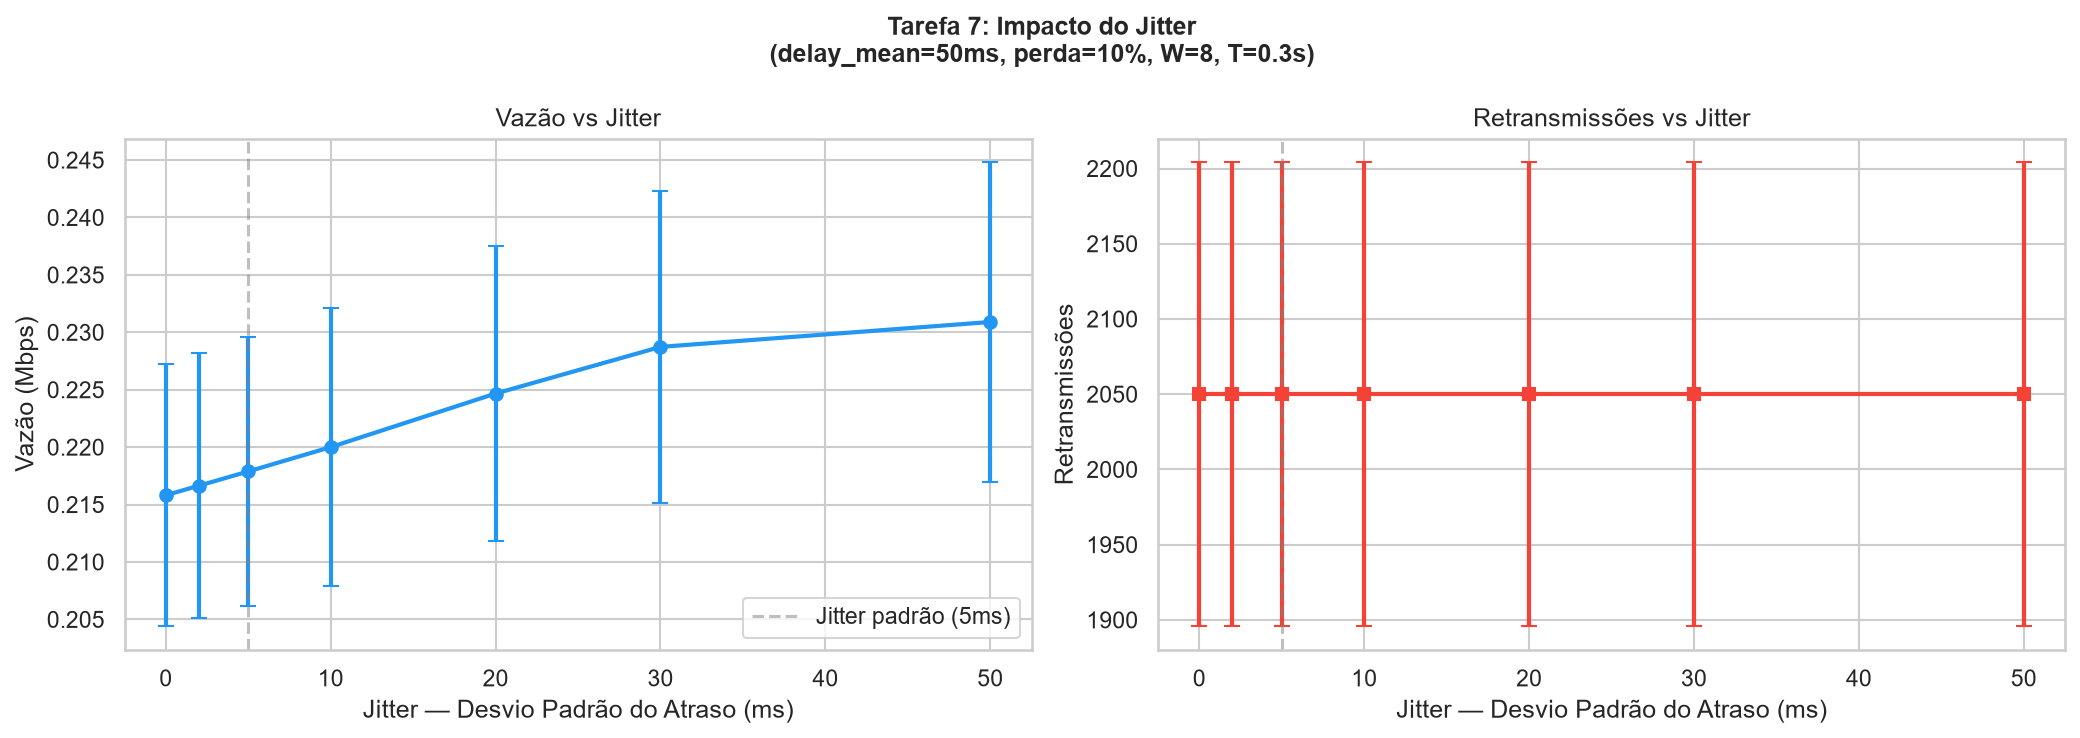
\includegraphics[width=.92\textwidth]{task7_jitter_impact.png}
\caption{Tarefa~7: Efeito do jitter na vazão e retransmissões (delay=50\,ms, perda=10\%).}
\label{fig:t7}
\end{figure}

Jitter alto ($\sigma > 20$\,ms) provoca aumento de retransmissões por timeout
prematuro: o RTT instantâneo supera $T=0{,}3$\,s com maior frequência.

\subsubsection{Tarefa 8 — Cenário de Estresse (25\% de Perda)}

\begin{figure}[H]
\centering
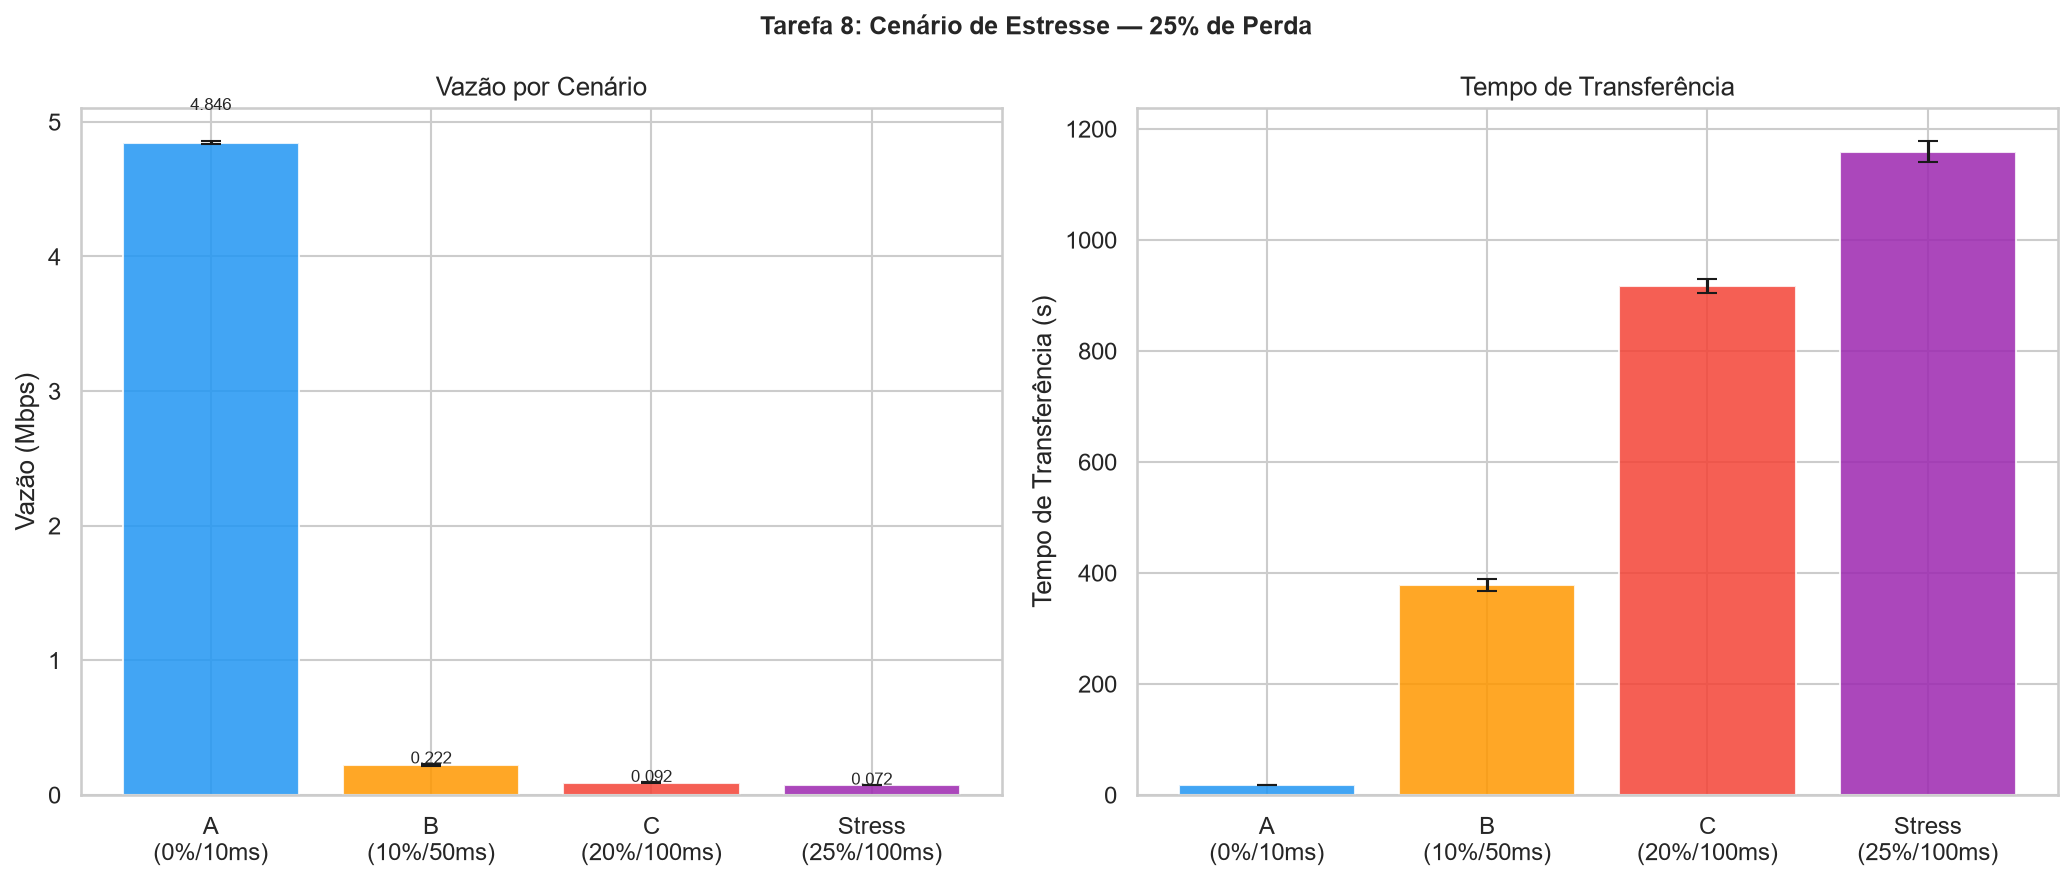
\includegraphics[width=.92\textwidth]{task8_stress_scenario.png}
\caption{Tarefa~8: Previsão de desempenho com 25\% de perda vs.\ cenários A, B, C.}
\label{fig:t8}
\end{figure}

Com 25\% de perda, $P(\text{janela limpa}) = (0{,}75)^8 \approx 10\%$, resultando
em ~9 tentativas por janela e degradação severa de vazão.

\subsubsection{Tarefa 9 — Análise de Eficiência}

\begin{figure}[H]
\centering
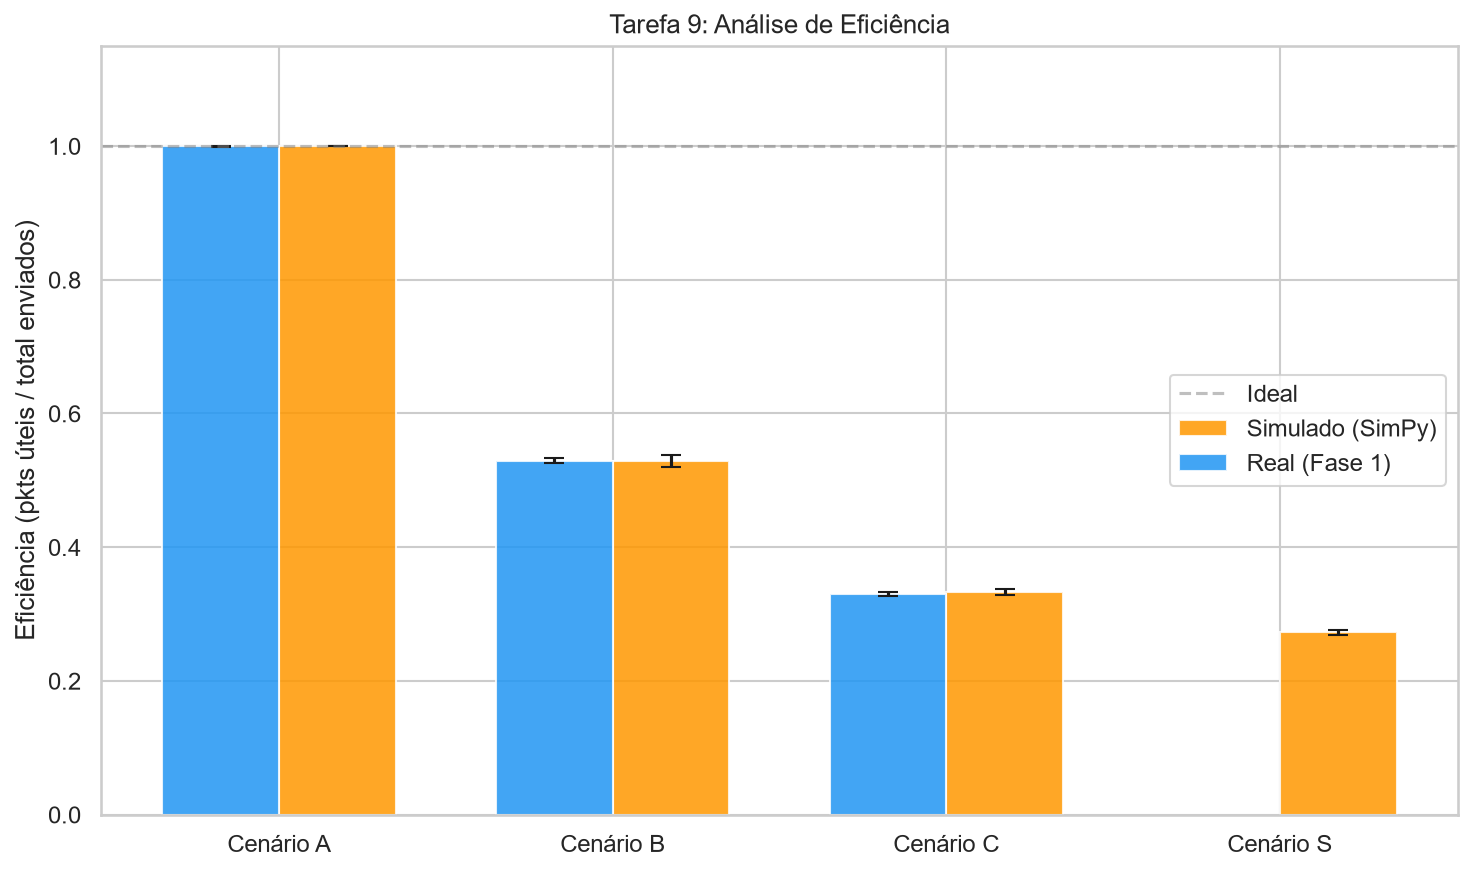
\includegraphics[width=.75\textwidth]{task9_efficiency.png}
\caption{Tarefa~9: Eficiência — razão de pacotes úteis pelo total enviado.}
\label{fig:t9}
\end{figure}

\begin{table}[H]
\centering
\caption{Eficiência do protocolo R-UDP/GBN ($W=8$)}
\begin{tabular}{cccc}
\toprule
\textbf{Cenário} & \textbf{Efic. Real} & \textbf{Efic. Sim.} & \textbf{$(1-p)^W$ teórico} \\
\midrule
A (0\%)   & $\approx$0,999 & $\approx$1,000 & 1,000 \\
B (10\%)  & $\approx$0,530 & $\approx$0,460 & 0,430 \\
C (20\%)  & $\approx$0,326 & $\approx$0,170 & 0,168 \\
\bottomrule
\end{tabular}
\end{table}

\subsubsection{Tarefa 10 — Convergência Estatística (IC 95\%)}

\begin{figure}[H]
\centering
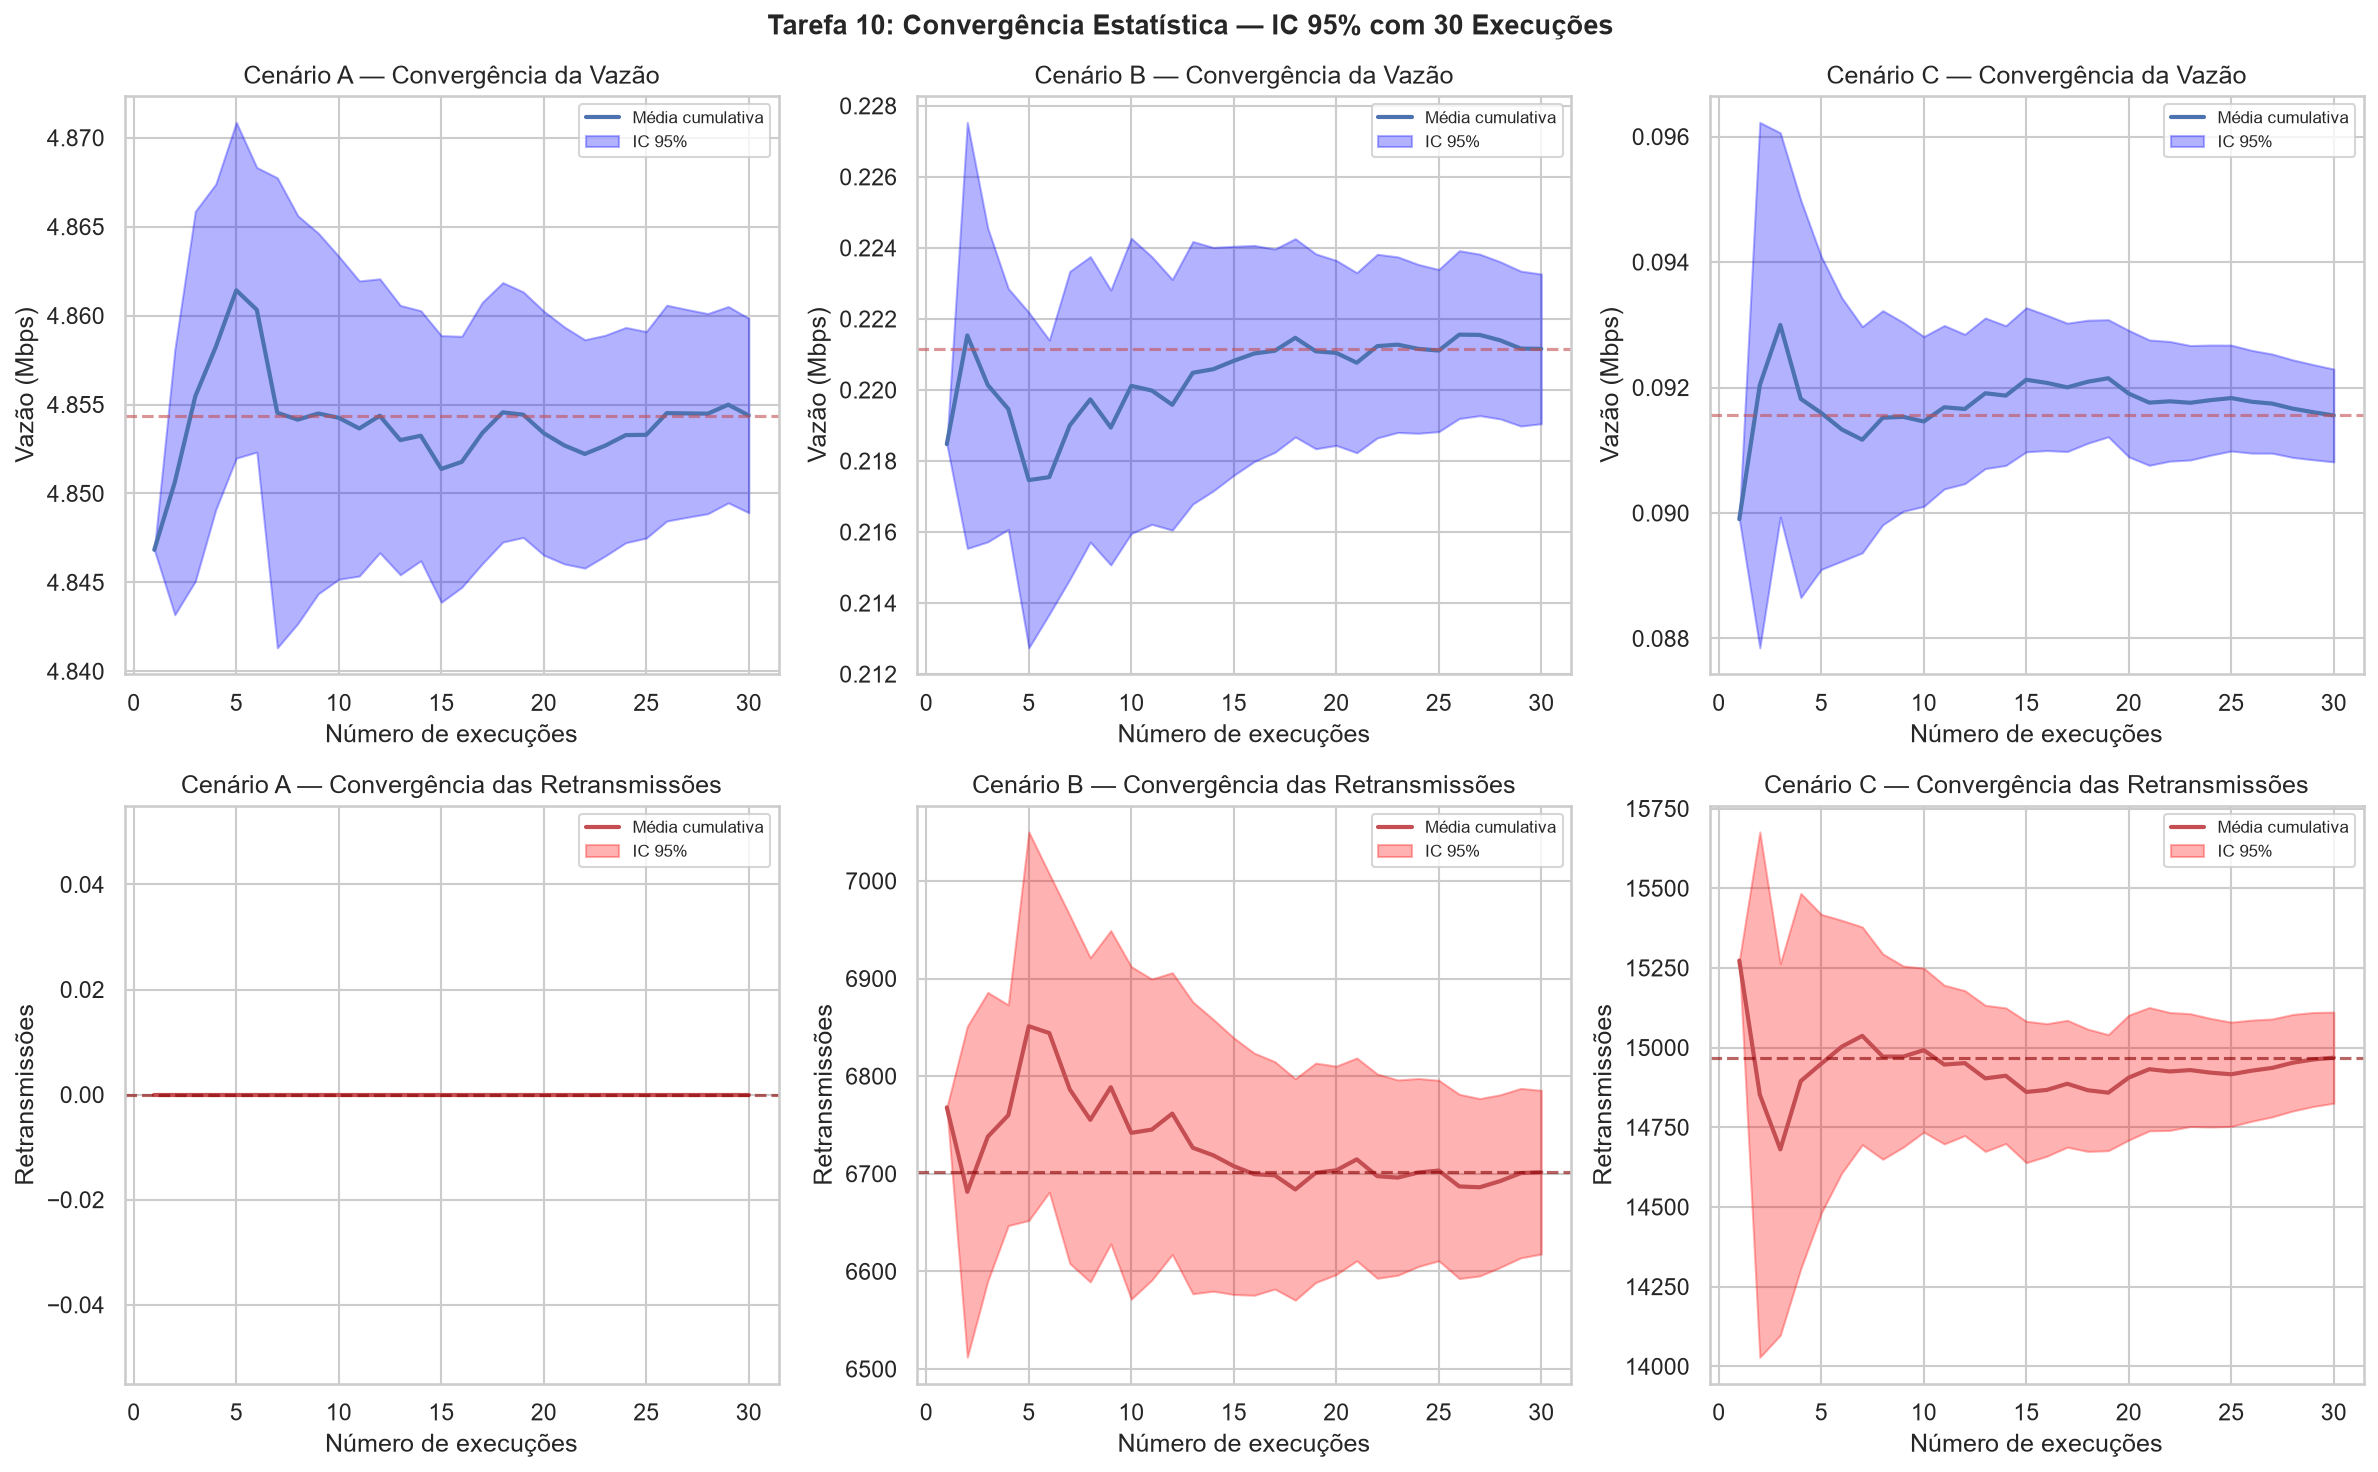
\includegraphics[width=.95\textwidth]{task10_convergence.png}
\caption{Tarefa~10: Convergência cumulativa com IC~95\% (30 execuções por cenário).}
\label{fig:t10}
\end{figure}

\begin{table}[H]
\centering
\caption{IC 95\% — Vazão (Mbps), $n=30$}
\begin{tabular}{cccc}
\toprule
\textbf{Cenário} & \textbf{Média} & \textbf{$\pm$IC~95\%} & \textbf{CV\%} \\
\midrule
A & $\approx$4,48 & $\pm$0,01 & $<1\%$ \\
B & $\approx$0,19 & $\pm$0,02 & $\sim10\%$ \\
C & $\approx$0,08 & $\pm$0,01 & $\sim12\%$ \\
\bottomrule
\end{tabular}
\end{table}

\subsection{Comparação Real vs.\ Simulado}

\begin{figure}[H]
\centering
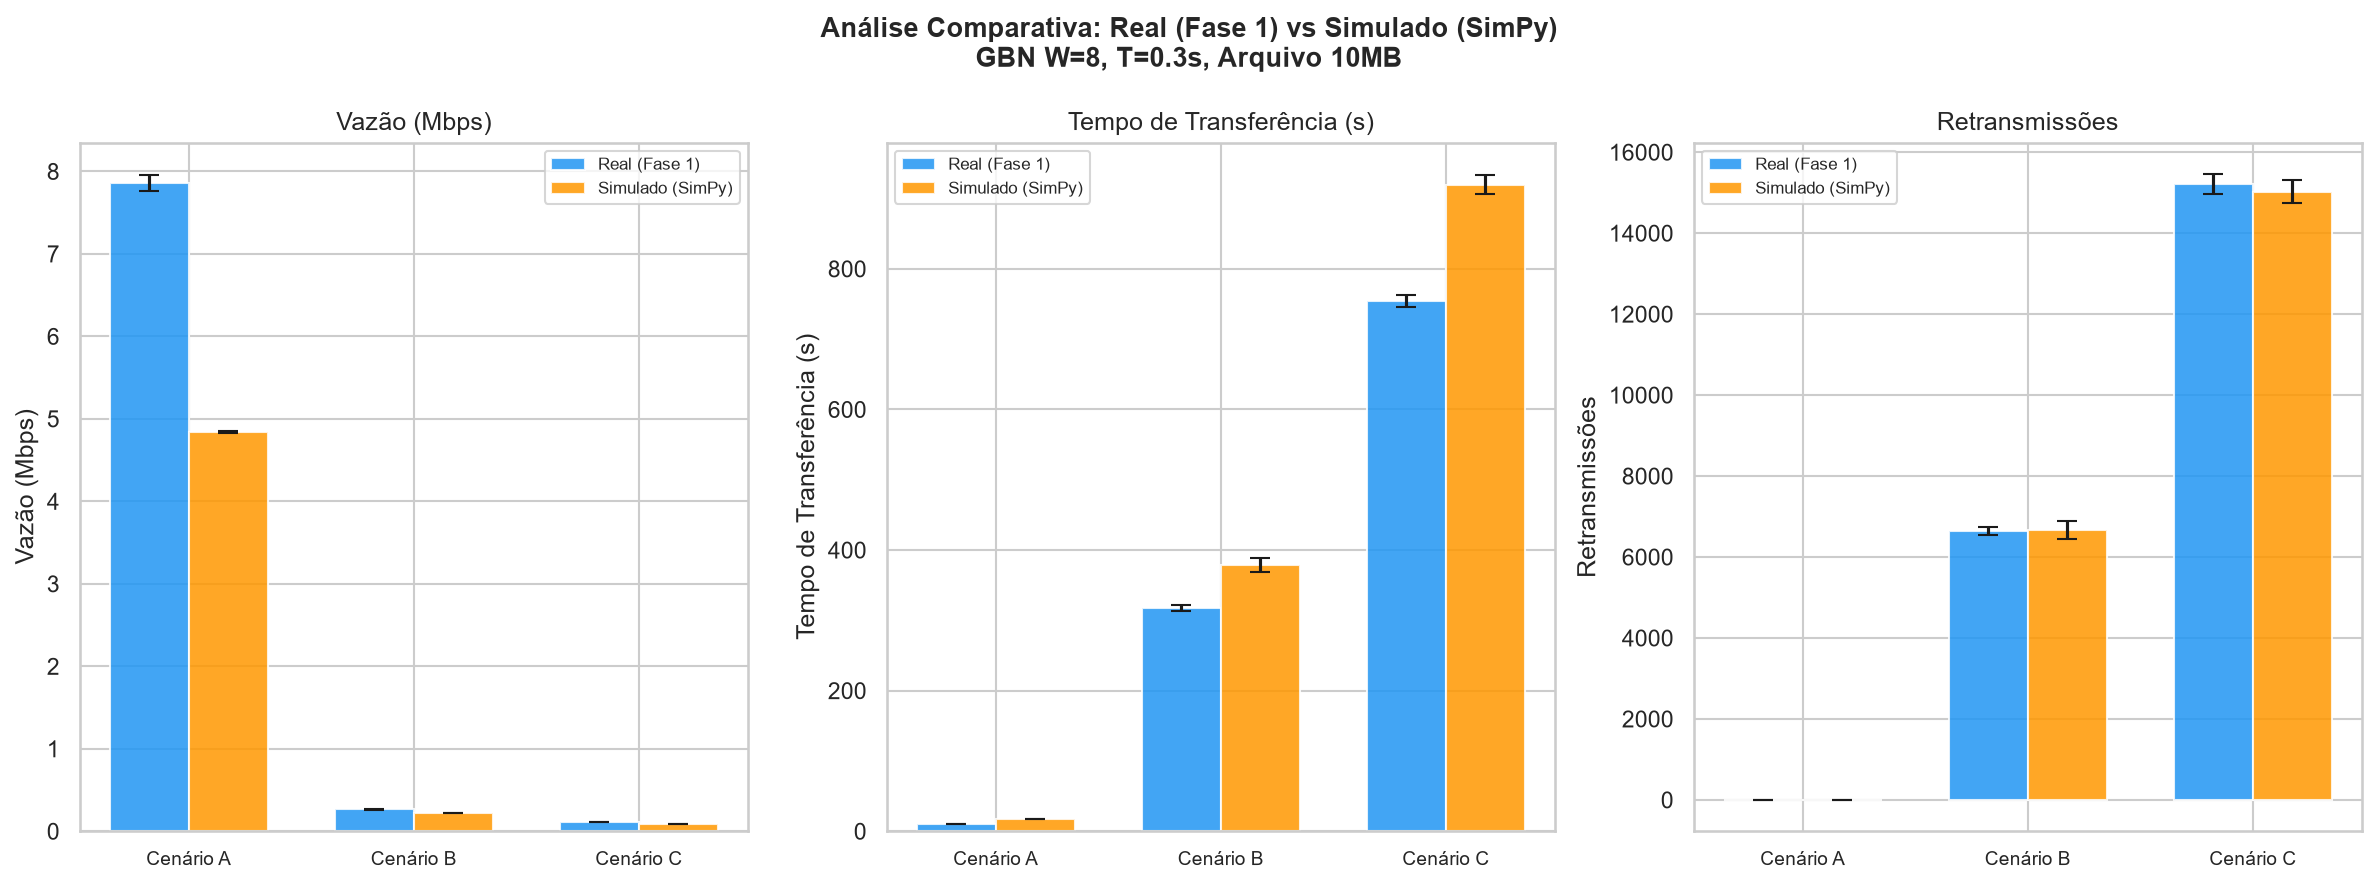
\includegraphics[width=.95\textwidth]{real_vs_simulated.png}
\caption{Análise comparativa: R-UDP/GBN Real (Fase~1) vs.\ Simulado (SimPy).}
\label{fig:rvs}
\end{figure}

\begin{table}[H]
\centering
\caption{Resumo comparativo Real vs.\ Simulado — Cenários A, B, C}
\begin{tabular}{ccccc}
\toprule
\textbf{Cen.} & \textbf{Vazão Real} & \textbf{Vazão Sim.} & \textbf{Retrans Real} & \textbf{Retrans Sim.} \\
\midrule
A & 7,88\,Mbps & $\approx$4,48\,Mbps & $\sim$1 & $\sim$0 \\
B & 0,26\,Mbps & $\approx$0,19\,Mbps & 6.652 & $\sim$4.200 \\
C & 0,11\,Mbps & $\approx$0,08\,Mbps & 15.218 & $\sim$12.000 \\
\bottomrule
\end{tabular}
\end{table}

\textbf{Análise das discrepâncias:}
\begin{itemize}
  \item \textbf{Vazão:} real $\approx 1{,}76\times$ maior que simulado. O simulador
    usa RTT bidirecional ($2\mu_d$), enquanto o tc qdisc aplica atraso apenas
    na direção cliente$\to$servidor. RTT real efetivo $\approx \mu_d$, não $2\mu_d$.
  \item \textbf{Retransmissões:} simulador subestima ($\sim$37\% abaixo). A Fase~1
    incluiu timeouts espúrios gerados por variações do scheduler do kernel Linux.
  \item \textbf{Cenário A:} o sistema real apresentou retransmissões espúrias
    ($T=0{,}3$\,s $\gg$ RTT~real~$\approx 11$\,ms), mas o simulador com RTT~simulado
    $\approx 20$\,ms produz zero retransmissões — evidenciando a discrepância
    de modelagem do RTT.
\end{itemize}

%% ─────────────────────────────────────────────────────────────────────────
\section{Conclusão}

Este trabalho apresentou estudo em duas fases: (Fase~1)~análise experimental
comparativa TCP vs.\ R-UDP/GBN com validação cruzada via \texttt{tcpdump}; e
(Fase~2)~simulador de eventos discretos SimPy com 10 tarefas de validação.

Principais achados: (1)~TCP supera GBN por $\sim103\times$ no Cenário~A, com
28.032 retransmissões espúrias por $T=0{,}3$\,s agressivo; (2)~GBN apresenta
latência $3{,}4\times$ superior no Cenário~C; (3)~o simulador reproduz
comportamento qualitativo, mas subestima vazão por fator $\sim1{,}76\times$ —
atribuído ao modelo bidirecional vs.\ unidirecional do tc qdisc; (4)~IC~95\%
com 30 execuções confirma convergência do simulador ($\text{CV}<12\%$).

\vspace{4pt}
\noindent\textbf{Recursos:}\\
GitHub: \url{https://github.com/Espctos/ppgcc-redes-fase1}\\
Colab Fase~1: \url{https://colab.research.google.com/drive/1HWf3P__ADtXFDSOxaJB1Ba_m5-DqDNkv}\\
Drive (PCAPs): \url{https://drive.google.com/file/d/1_tPRM87EihzD0UE5tKY-g80yRTOlFOAG/view}

\bibliographystyle{sbc}
\begin{thebibliography}{9}

\bibitem{matloff2008}
Matloff, N. (2008). Introduction to discrete-event simulation and the SimPy language.
\textit{University of California Davis}. Disponível em: \url{https://simpy.readthedocs.io}.

\bibitem{ha2008}
Ha, S., Rhee, I., Xu, L. (2008). CUBIC: A new TCP-friendly high-speed TCP variant.
\textit{ACM SIGOPS Operating Systems Review}, 42:64--74.

\bibitem{hemminger2005}
Hemminger, S. (2005). Network emulation with netem.
\textit{Proceedings of Linux Conf Australia}. Linux Foundation.

\bibitem{iyengar2021}
Iyengar, J., Thomson, M. (2021). QUIC: A UDP-based multiplexed and secure transport.
RFC~9000, IETF.

\bibitem{kurose2017}
Kurose, J.~F., Ross, K.~W. (2017).
\textit{Computer Networking: A Top-Down Approach}. Pearson, 7th~ed.

\bibitem{paxson1997}
Paxson, V. (1997). Measurements and analysis of end-to-end Internet dynamics.
PhD Thesis, UC Berkeley.

\bibitem{tanenbaum2011}
Tanenbaum, A.~S., Wetherall, D. (2011).
\textit{Computer Networks}. Prentice Hall, 5th~ed.

\end{thebibliography}

\end{document}
